
\subsection{SHMR}
The SHMR for all the galaxies with $M_{*} > 10^10 M_{\odot}$ from TNG is plotted in figure \ref{shmr_res1}, along with the best fits from \cite{Moster2012} and \cite{Behroozi2013}.



\begin{figure}
    \centering
    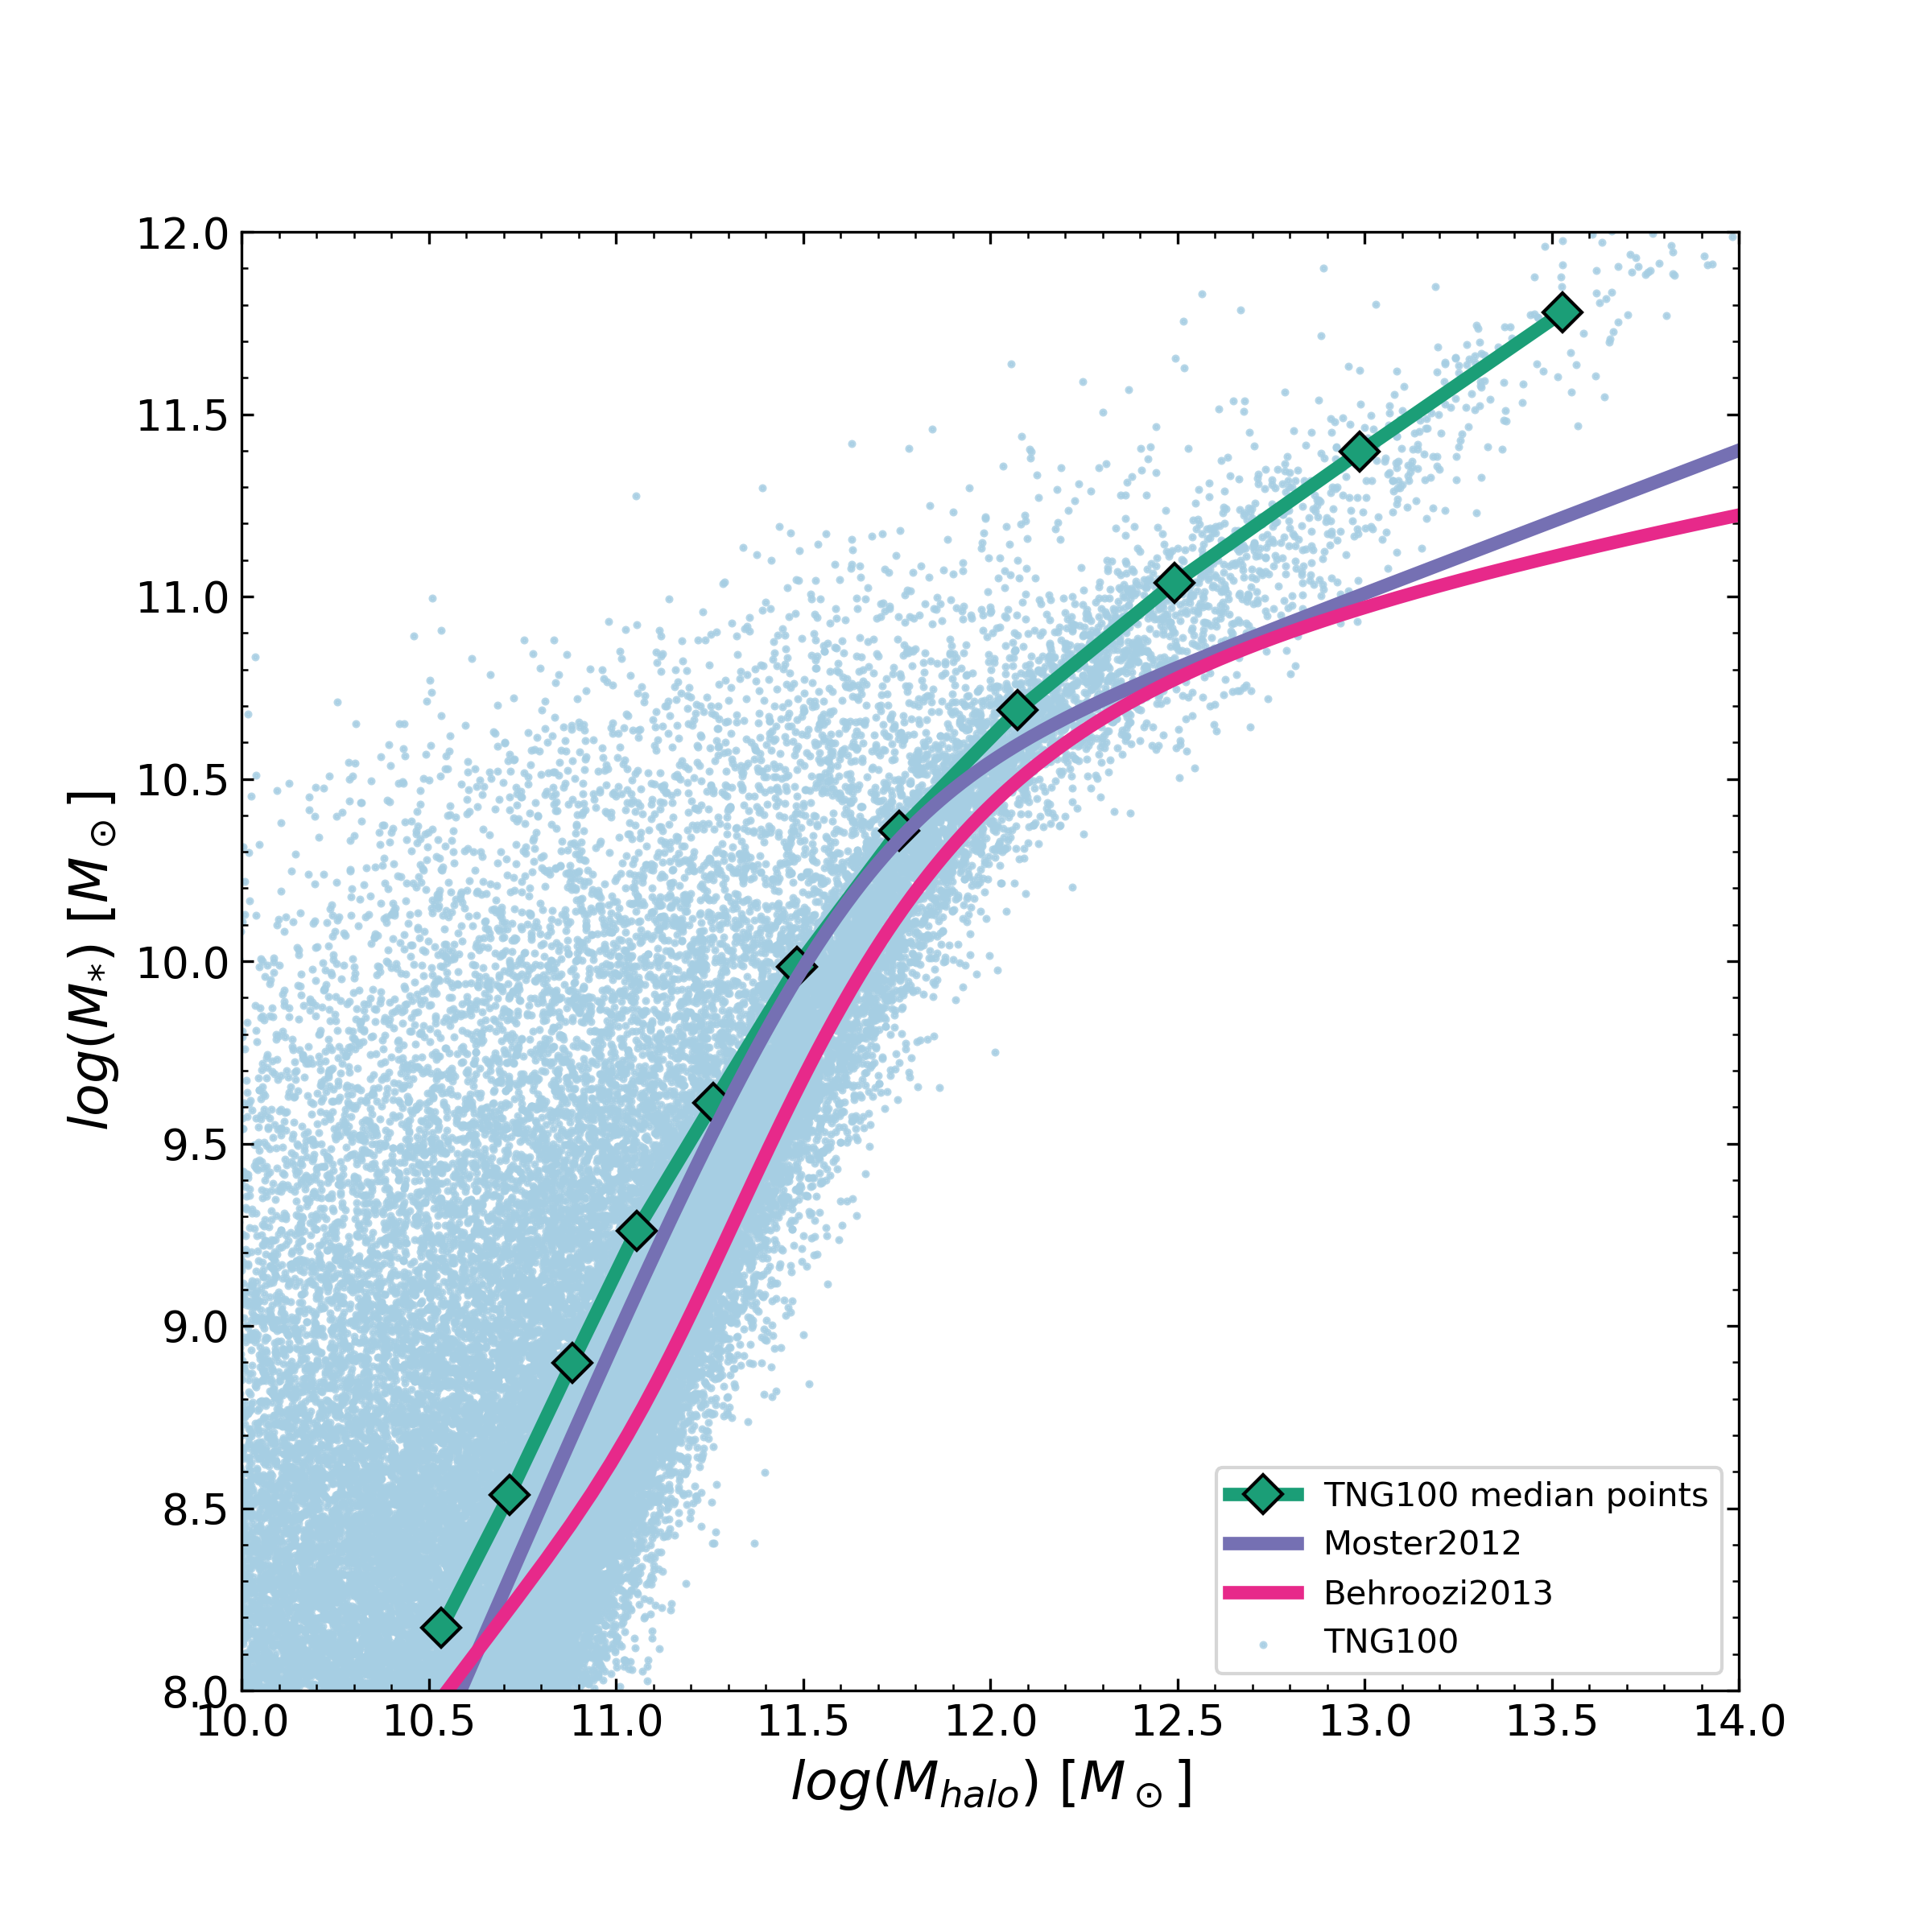
\includegraphics[width=0.9\textwidth]{images/results_shmr_all_galaxies.png}
    \caption{}
    \label{shmr_res1}
\end{figure}

\begin{figure}
    \centering
    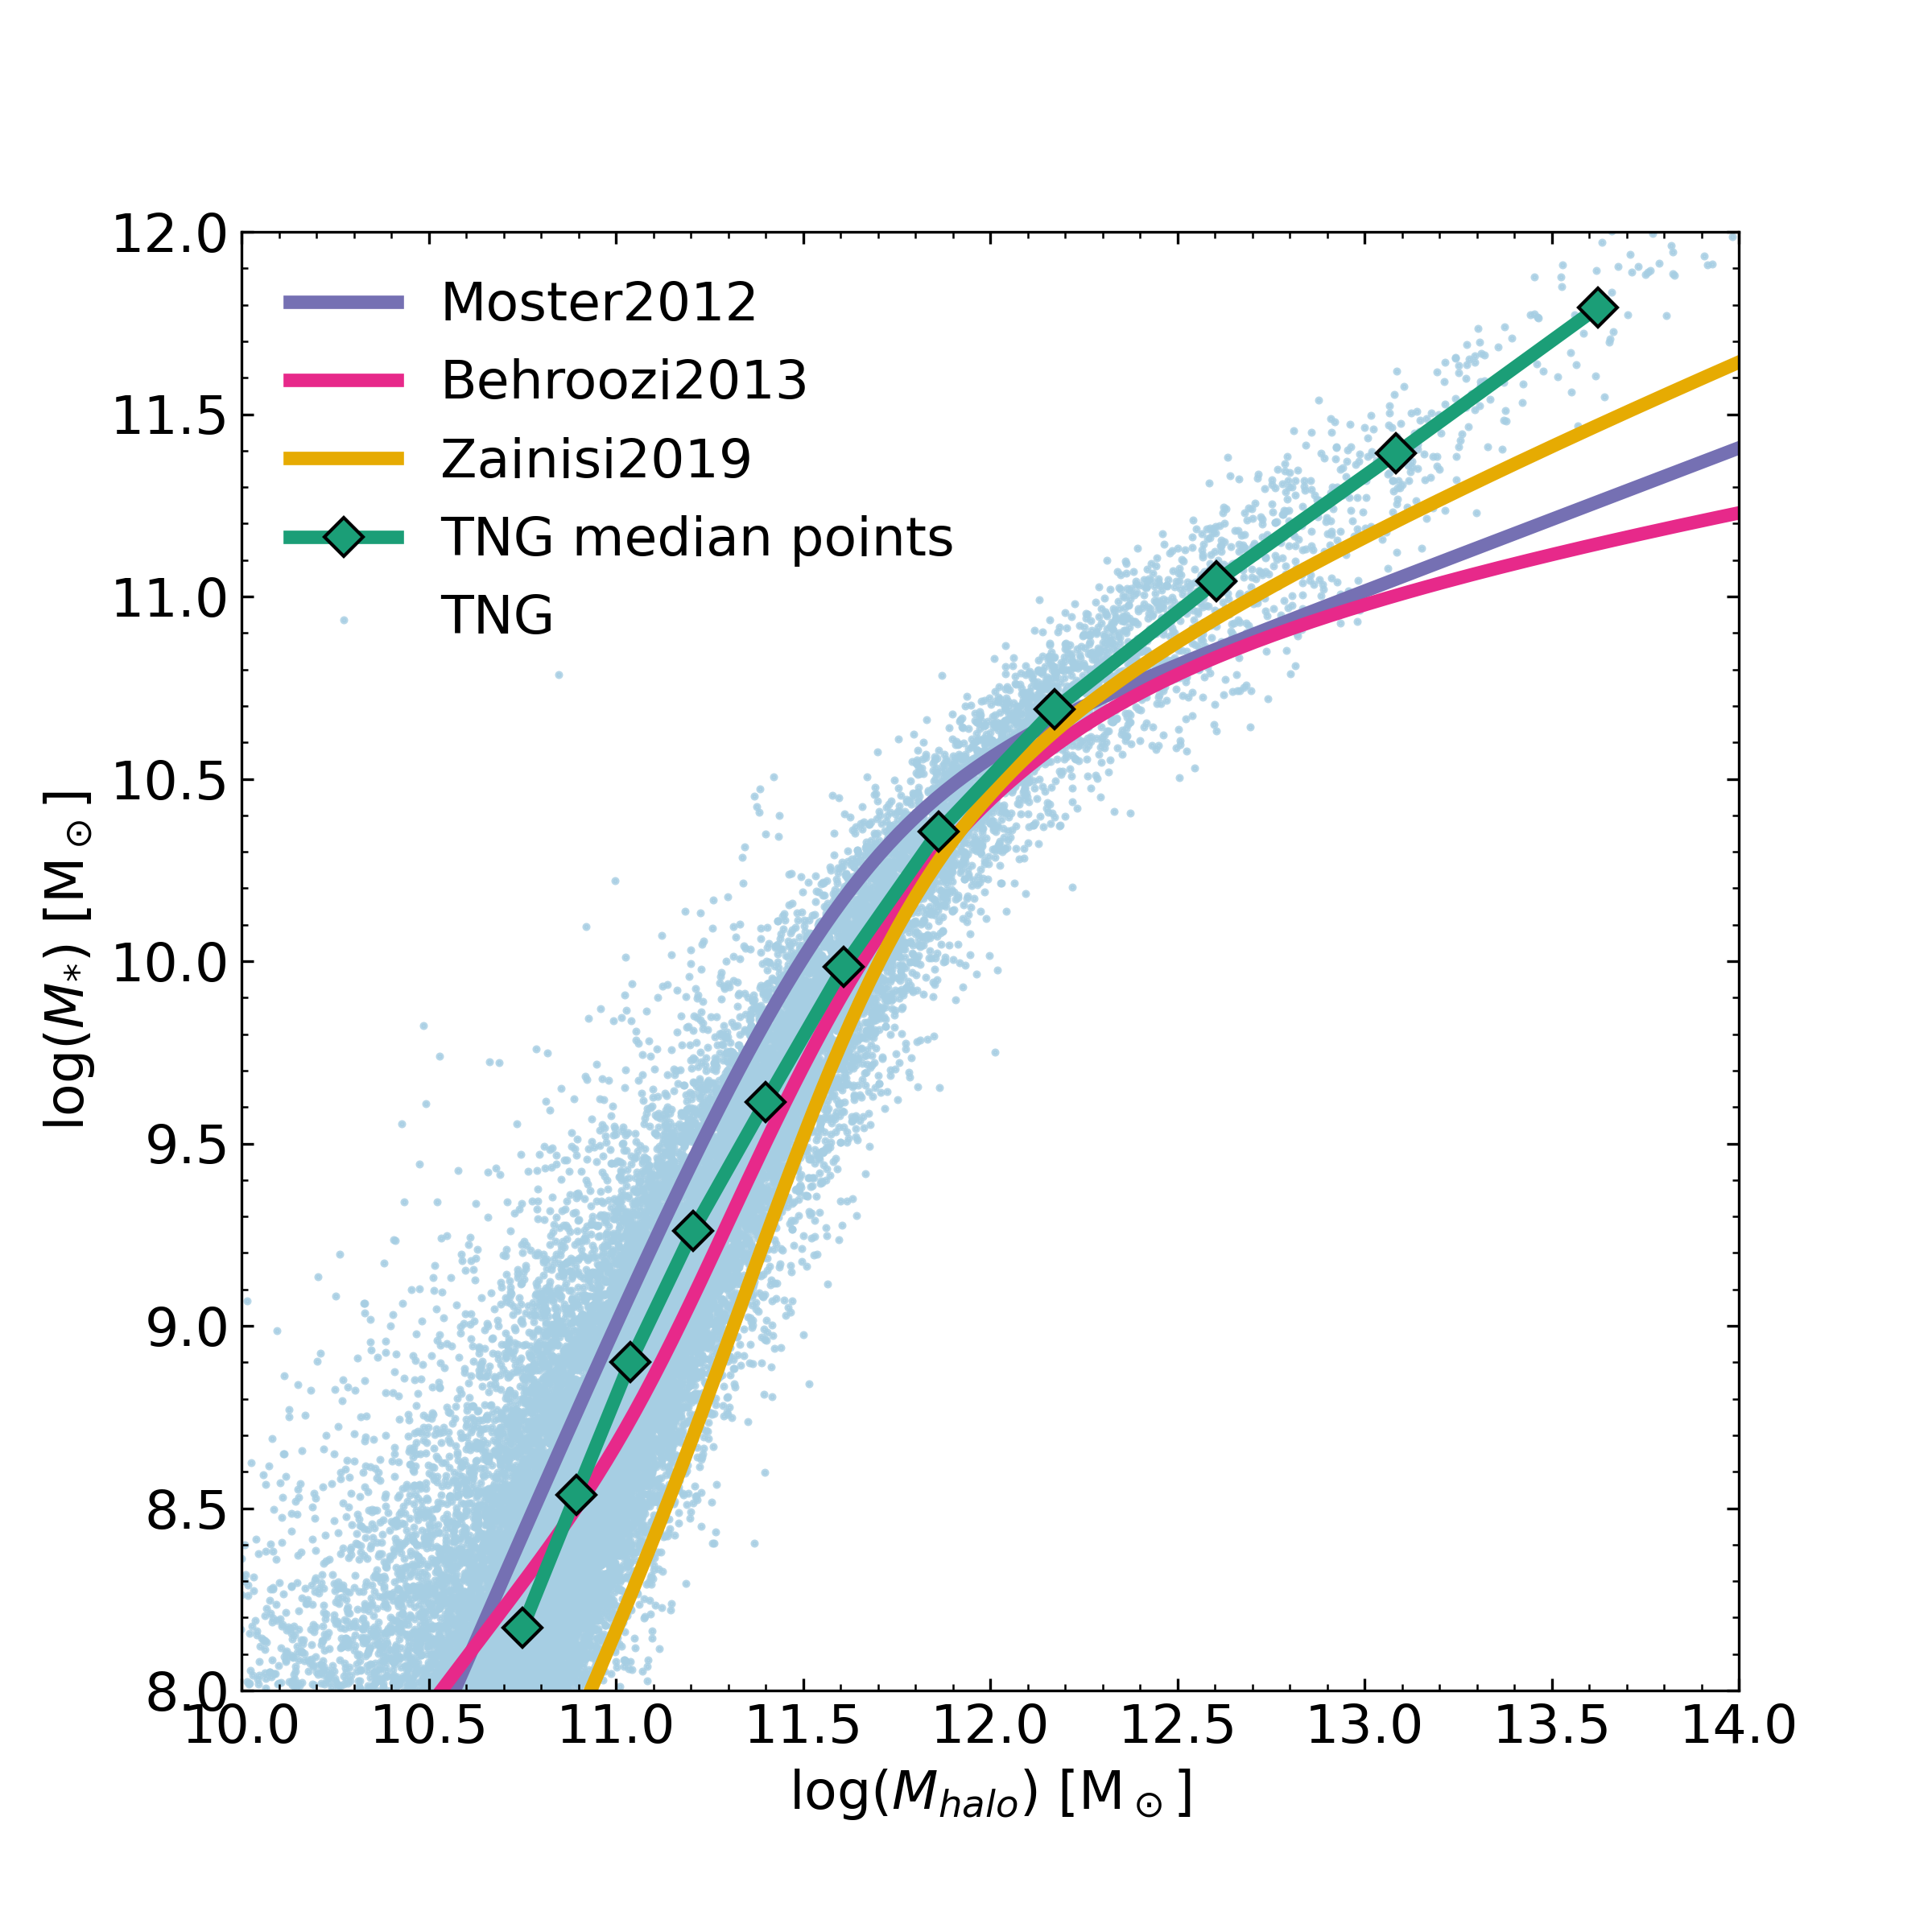
\includegraphics[width=0.9\textwidth]{images/results_shmr_central_galaxies.png}
    \caption{}
    \label{shmr_res2}
\end{figure}

\subsection{TFR}

\subsection{FJ relation and the FP}

%\begin{figure}
 %   \centering
 %   \includegraphics[width=\textwidth]{images/fj.png}
 %   \caption{Early type galaxies for both TNG and SAMI.}
 %   \label{FJ_results}
%\end{figure}

%The velocity dispersion as function of stellar mass can be seen in Figure \ref{FJ_results}. The trend for the TNG-100 data is a clear power law as expected from the FJ relation. Compared to the observational data, the simulation data shows lower $\sigma$ values, by about 0.1-0.2 dex. This could be explained by the fact that the $\sigma$ in the TNG galaxies is averaged across all particles, across the whole size of the subhalo. In general, gas has a lower $\sigma$ than stars and dark matter, so this could push the total $\sigma$ down. However, in early-type galaxies there is little gas so the impact would be expected to be small. The fact that $\sigma$ is found by averaging across the entire subhalo would include particles further out than for the SAMI data in which the velocity dispersion is averaged inside the effective radius ($\sigma_{e}$) is used. Other studies have also found that simulations tend to get lower values for $\sigma$ \parencite{Sande2018}, so this might also just be a limitation of the simulations.

\subsection{Color bimodality}

\subsection{SMBH relations}